\documentclass[12pt,letterpaper]{article}
\usepackage{natbib}

%Packages
\usepackage{pdflscape}
\usepackage{fixltx2e}
\usepackage{textcomp}
\usepackage{fullpage}
\usepackage{float}
\usepackage{latexsym}
\usepackage{url}
\usepackage{epsfig}
\usepackage{graphicx}
\usepackage{amssymb}
\usepackage{amsmath}
\usepackage{mathtools}
\usepackage{bm}
\usepackage{array}
\usepackage[version=3]{mhchem}
\usepackage{ifthen}
\usepackage{caption}
\usepackage{hyperref}
\usepackage{amsthm}
\usepackage{amstext}
\usepackage{enumerate}
\usepackage[osf]{mathpazo}
\usepackage{dcolumn}
\usepackage{lineno}
\usepackage{dcolumn}
\newcolumntype{d}[1]{D{.}{.}{#1}}

\pagenumbering{arabic}


%Pagination style and stuff
\linespread{2}
\raggedright
\setlength{\parindent}{0.5in}
\setcounter{secnumdepth}{0} 
\renewcommand{\section}[1]{%
\bigskip
\begin{center}
\begin{Large}
\normalfont\scshape #1
\medskip
\end{Large}
\end{center}}
\renewcommand{\subsection}[1]{%
\bigskip
\begin{center}
\begin{large}
\normalfont\itshape #1
\end{large}
\end{center}}
\renewcommand{\subsubsection}[1]{%
\vspace{2ex}
\noindent
\textit{#1.}---}
\renewcommand{\tableofcontents}{}
%\bibpunct{(}{)}{;}{a}{}{,}

%---------------------------------------------
%
%       START
%
%---------------------------------------------

\begin{document}

%Running head
\begin{flushright}
Version dated: \today
\end{flushright}
\bigskip
\noindent RH: Branch swapping algorithm

\bigskip
\medskip
\begin{center}

\noindent{\Large \bf Tree rearrangements rearranged} %TG: I'm bad at puns.
\bigskip

\noindent {\normalsize \sc Thomas Guillerme$^1$$^*$, and Martin D. Brazeau$^1$}\\ %TG: Author order can be swapped of course! There's only a finite combination of 2 elements anyway!
\noindent {\small \it 
$^1$Imperial College London, Silwood Park Campus, Department of Life Sciences, Buckhurst Road, Ascot SL5 7PY, United Kingdom.\\}
\end{center}
\medskip
\noindent{*\bf Corresponding author.} \textit{t.guillerme@imperial.ac.uk}\\  %TG: Same as above
\vspace{1in}

%Line numbering
\modulolinenumbers[1]
\linenumbers

%---------------------------------------------
%
%       ABSTRACT
%
%---------------------------------------------

\newpage
\begin{abstract}
blablabla
\end{abstract}

\noindent (Keywords: )\\

\vspace{1.5in}

\newpage 


%---------------------------------------------
% LaTeX tips for modifying/editing the document:
%---------------------------------------------
% - You can comment using the percentage sign. I suggest you use the % sign alone for commenting out sections of the text:
%       e.g. "This is a really long sentence %because this sentence is very long." Here the % is used for ignoring the end of the sentence (but for some reason you want to keep track of it).%
%       For comments as in verbose comments, I suggest you use "%MB:":
%       e.g. "This is a really long sentence %because this sentence is very long. %MB: yeah, no shit!" 
% - For optimal version control, write only one sentence per line (for more precise track changes)
% - To build the pdf, use command+B in Sublime.
% - Because of the bibliography, the pdf needs to be build in the same folder that contains "References.bib" and "sysbio.bst"
% - For citing papers, you must put their bibtex reference in the "References.bib" file and then you can use the following sysbio tags:
%        \cite{bibtexBob2000} for citing within a sentence: "Bob (2000)"
%        \citep{bibtexBob2000} for citing within brackets: "(Bob, 2000)"
%        \citep[Before:][-After]{bibtexBob2000} for citing within brackets with additional text: "(Before: Bob, 2000 -After)"
%        \citealt{bibtexBob2000} for citing without brackets: "Bob, 2000"
%        You can put more cites in each \cite tag by separating them with commas.
% - For equation, find every details here: https://en.wikibooks.org/wiki/LaTeX/Mathematics
% - For titles and stuff, the hierarchy goes \section{}, \subsection{}, \subsubsection{} and so forth...
% - For bullet points or enumerations you can use:
%       \begin{itemize}
%           \item my first bullet point/enumeration
%       \end{itemize}
%       With replacing "itemize" by "enumerate" for enumeration.




%---------------------------------------------
%
%       INTRODUCTION
%
%---------------------------------------------
\section{Introduction}

% Tree rearrangement is paramount
Phylogenetics, as the way to infer the relations between organisms, is at the base of literally every endeavour in modern biology ans has also important ramifications outside of biological sciences \citep[e.g. linguistics;][]{Bouckaert24082012}.
Although many of the methods related phylogenetics, ranging from gene alignments \citep[e.g.][]{Tan01092015} to tree comparisons \citep[e.g.][]{kuhner2015treComparison} are widely studied, used and taught \citep{desalle2012phylogenomics}, one crucial aspect, tree rearrangement methods, is often ignored or over-looked by most biologists.
In fact, these methods are used during crucial steps of the phylogenetic inference procedure (i.e. ``building'' the trees) since they allow to efficiently explore the tree space \citep[see ][]{Sanderson448} in search for the best topology, whether based on optimality criteria \citep[e.g. maximum parsimony; ][]{swofford2003paup} or probabilistic methods \citep[e.g. likelihood or Bayesian; ][]{Stamatakis21012014,Ronquist2012mrbayes}.
Moreover, tree rearrangement methods are also at the base of some post tree inference tasks such as tree comparisons \citep[e.g.][]{allen2001subtree,kuhner2015treComparison}, node support estimation \citep[e.g.][]{goloboff2014bias} or specific analysis such as horizontal genes transfer \citep[e.g.][]{mcfadden1995something,bordewich2005computational} to cite only a few.

% Because of the shit ton of trees
In phylogenetic inference, tree rearrangement methods (or branch swapping) is used to explore tree space \citep[i.e. the realm of all the possible trees][]{page1993islands,morrison2007increasing,Sanderson448}.
In practice, this tree space can easily be astonishingly big.
For example, considering the topology parameter only, the number of topologies that can be obtained with any tree with $n$ number of taxa is $(2n-3)!!$ for rooted trees and $(2n-5)!!$ for unrooted ones.
To put it in perspectives, for only 14 taxa, the tree space contains more than a trillion topologies ($7.9\times10^{12}$)!
Thus, one of the major challenge in tree rearrangement methods is to find a fast and reliable algorithm that only visits a subset of these topologies to find the optimal topology. 
The speed of the tree rearrangement can be solved by efficient algorithm implementation (e.g. algorithms that require a low amount of memory by using ring-based tree structures)[CITE].
Conversely, the reliability aspect must be based on strict rules in the algorithm avoiding unwanted tree rearrangements \citep{allen2001subtree,felsenstein2004inferring,lakner2008efficiency,goloboff1993character}.

% Also these algorithms can have some caveats
Two main points need to be considered for the reliability of tree arrangement algorithms:
\begin{enumerate}
    \item First, when the tree search only visits some possible solutions this can create problems by having a higher probability of visiting a specific tree topology island since the probability of obtaining any topology by tree rearrangement will not be equal (some topologies might be more visited by chance).
    More concretely, for a tree with $n$ taxa, tree rearrangement algorithms can produce $M$ topologies including $m$ similar ones.
    If the tree search algorithm is set to subsample $m$ topologies only, it can possibly only subsample the $m$ similar topologies thus being literally ineffective at exploring tree space \citep{allen2001subtree}.
    \item Second, the order in which the possible tree rearrangement topologies are visited is also paramount.
    In fact, to avoid any statistical bias, the visiting order should be strictly random \citep{goloboff2014bias} although, in practice, and for algorithm speed reasons, this is rarely the case (e.g. using post/pre-order traversals [CITE]).
    This as been shown to introduce several biases in theoretical examples \citep{goloboff2014bias} although, to our knowledge, has not been demonstrated empirically.
\end{enumerate}

% We therefore need some good algorithms.
Solutions have been proposed by people in forms of different algorithm implementation that avoid redundant topologies to be visited \citep{allen2001subtree} and that these topologies are visited randomly \citep{goloboff2014bias}.
Two of the most popular algorithms are the Subtree Pruning and Regrafting method (SPR) and the Tree Bisection and Reconnection method \citep[TBR - see Fig. \ref{Figure_SPR} and \ref{Figure_TBR} and text below for detailled description;][]{allen2001subtree,felsenstein2004inferring}.
These two algorithms are often considered separately since they produce different series of tree rearrangements: SPR produces more closely related trees than TBR.
However, in practice, the efficiency of those algorithms for finding the best topology varies in function of the method, the data and their combination with other tree rearrangement algorithms \citep[e.g.][]{morrison2007increasing,lakner2008efficiency}.
Also the way the trees are visited (see point 2 above) modifies the efficiency of these algorithms.
For example, \cite{lakner2008efficiency} found, for Bayesian inference, that SPR (when sampled randomly) was more efficient than TBR (when sampled non-randomly) which was in turn more efficient than SPR (when sampled non-randomly).

The tree inference literature contains thorough and precise descriptions of both the algorithms \citep[e.g.][]{allen2001subtree,felsenstein2004inferring} and their caveats \citep[i.e speed and reliability - e.g.][]{morrison2007increasing,lakner2008efficiency,goloboff2014bias}.
However, the \textit{implementation} of the algorithms is often overlooked.
Here, we will review two common branch rearrangement algorithms (SPR and TBR) and propose a more practical and intuitive definition of the algorithms that we believe can help their implementation.
It is important to note that the algorithms described here are mathematically equivalent to the ones described in \cite{allen2001subtree} and \cite{felsenstein2004inferring} and we thus do not claim priority or originality on this method that as certainly already be implemented in many softwares and was ``discovered'' empirically by many coders.
%TG: add something about writing code for humans not computers? (i.e. non-cryptic/obfuscating coding practices)

\section{SPR and TBR described in literature}

% \subsection{Tree elements definition}
% \begin{itemize}
%     \item a \textbf{tip} is any leaf of the tree (degree 1 vertices) that is connected to only one node.
%     \item a \textbf{node} is formed by the connection of tips or nodes. In a binary tree, a node has exactly one ancestor (or parent) and two descendants.
%     \item an \textbf{edge} is any single connection between two nodes or a node and a tip.
%     \item the \textbf{root} is the single edge that is only connected to one node (and nothing).
% \end{itemize}
% Any bifurcating (i.e. fully resolved) tree with $n$ tips has $2n-1$ nodes and $2n-2$ edges ($n-2$ internal ones) if rooted and $2n-2$ nodes and $2n-3$ edges ($n-3$ internal ones) if unrooted.

% Definitions: \cite{allen2001subtree,felsenstein2004inferring}

\subsubsection{Subtree Pruning and Regrafting (SPR)}
This method consists in removing any subtree from the original tree (including all trees with only one tip and one edge, i.e. the individual tips) and reinserting it along every edges back on the original tree \citep[see Fig \ref{Figure_SPR} and ][]{felsenstein2004inferring}.
In other words, a tree with $n$ taxa, is split into two trees: the target tree with $n_{target}$ taxa and the subtree with $n_{subtree}$ taxa (where $n_{subtree} \geq 1$).
The substree is then reinserted in the $(2n_{target}-3)$ positions available on the target tree \citep{felsenstein2004inferring}.
Thus, the total number of SPR rearrangements for an original tree with $n$ taxa is $4(n-3)(n-2)$.
Redundant tree topologies occur when the subtree is regrafted (or rebranched) on it's original position and on one of the neighbouring edge to it's original position \citep{allen2001subtree}.

% The number of SPR rearrangements to cover all topologies without redundant swaps as:
% \begin{equation}
%     \text{Total SPR}={\overbrace{(2n-3)}^{\text{edges}}} {\overbrace{(2n-4)}^{(\text{edges} - 1)}} % TG: or use \sum{SPR}?
% \end{equation}
% Where $(2n-3)$ is the number of subtrees one can obtain from an original $n$ taxa tree and $(2n-4)$ are the number of reinsertions possible from these subtrees on the target trees \cite{allen2001subtree}.

From this total, we can remove the $6(n-2)$ resulting trees corresponding to regrafting the subtrees on the edge where the subtree was pruned from \citep[i.e. the rearrangements resulting in the same topology; ][]{allen2001subtree}, and the $8(n-3)$ resulting trees corresponding to regrafting the subtrees on the edge adjacent to the pruned edge \citep{allen2001subtree}.
Thus the number of unique topologies obtained by SPR is $4(n-3)(n-4)$.

\begin{figure}[!htbp]
\centering
   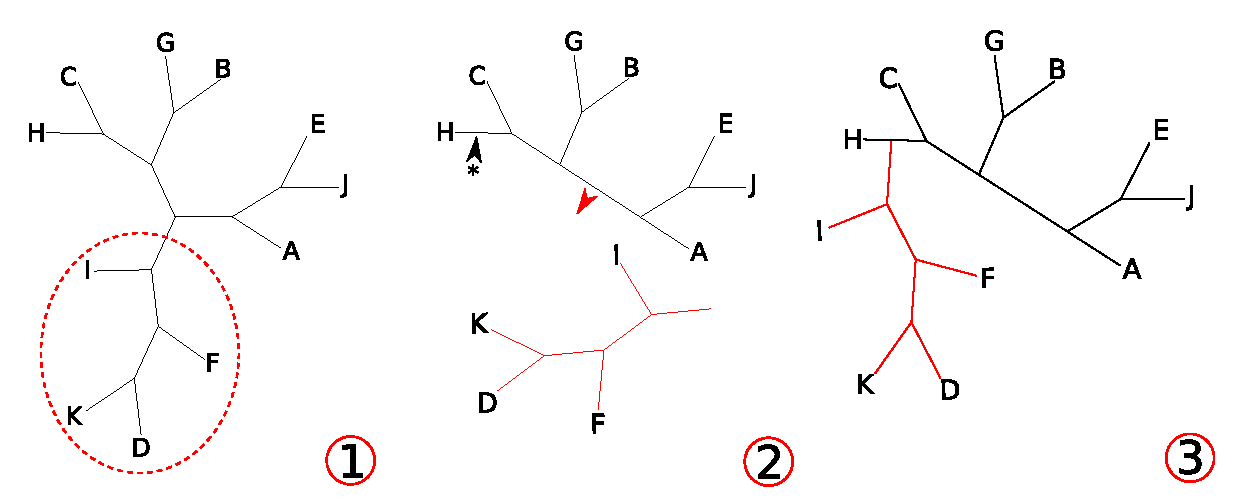
\includegraphics[width=0.9\textwidth]{Figure/SPR.pdf}
\caption{Suptree Pruning and Regrafting (SPR). Modified from \cite{felsenstein2004inferring}, Figure 4.5. \textbf{1}: a random subtree with $n$ tips is selected; \textbf{2}: the red arrow designates the edge where the subtree was previously branched and the black one the new insertion point. Note that all the edges but the one with the red arrow are potential insertion points. \textbf{3}: the new topology obtained by one SPR rearrangement.}
\label{Figure_SPR}
\end{figure}

\subsubsection{Tree Bisection and Reconnection (TBR)}
This method consists in breaking the original tree into two distinct subtrees (the bisection).
The first subtree is then sequentially rerooted on each of its edges and then rebranched on every edges of the second subtree (the reconnection).
For a tree with $n$ taxa separated into two trees with $n_{1}$ taxa and $n_{2}$ taxa, there will be $(2n_{1}-3)(2n_{2}-3)$ possible ways to recombine the them \citep{felsenstein2004inferring} with $n_{1}$ and $n_{2}$ ranging from $2$ to $n-2$ depending on the tree's topology.

% This operation can be repeated for all the internal edges in the original tree, thus the maximum TBR can be:
% \begin{equation}
%     \text{Maximum TBR} = \overbrace{(n-3)}^{\text{internal edges}} \sum_{i=2}^{n-2} (2i-3)(2(n-i)-3) %TG: Check! Summation might be incorrect
% \end{equation}
% Where $i$ and $n-i$ corresponds respectively to the size of the smallest and biggest trees resulting from the bisection the original tree.

\begin{figure}[!htbp]
\centering
   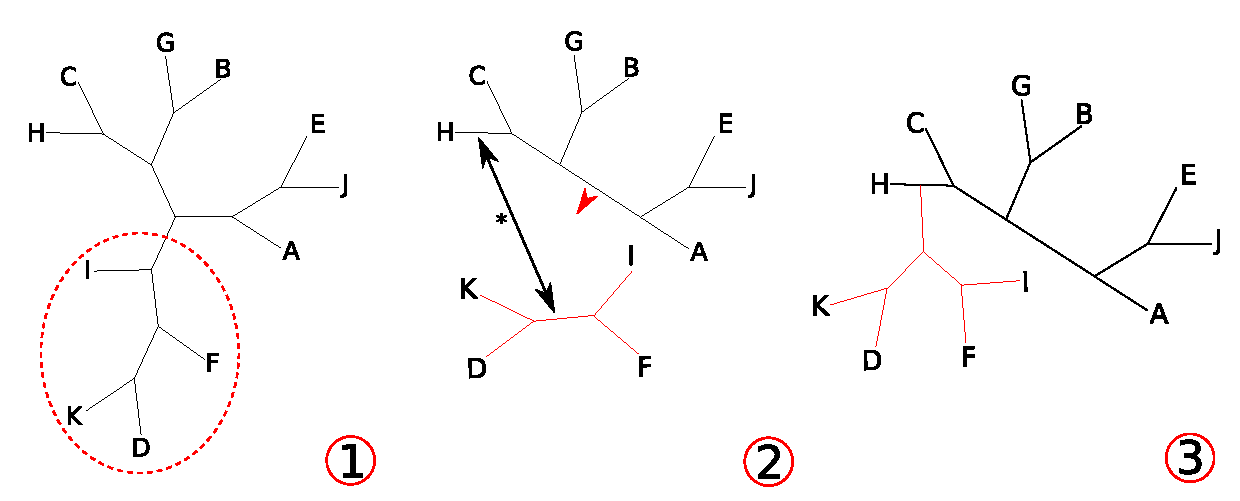
\includegraphics[width=0.9\textwidth]{Figure/TBR.pdf}
\caption{Tree Bisection and Reconnection (TBR). Modified from \cite{felsenstein2004inferring}, Figure 4.6. \textbf{1}: the trees are split at a random edge and both subtrees are unrooted; \textbf{2}: the red arrow designates the edge where the red tree was previously connected and the black one designates the new rooting point on the red tree and its insertion on the black tree. Note that all the edges on the black tree (but the one with the red arrow) are potential reconnection points. \textbf{3}: the new topology obtained by one TBR rearrangement.}
\label{Figure_TBR}
\end{figure}

\section{Implementation spin}
These two algorithms can be seen as technically different since they will produce different tree islands, for example, the SPR will, in theory explore less topologies than the TBR \citep[see above and][]{morrison2007increasing,lakner2008efficiency}.
However, once one excludes the visiting of redundant topologies in both algorithms, they can be seen as a generalised way to explore effectively all possible tree topologies.
First, as described in \cite{allen2001subtree} (but not in \citealt{felsenstein2004inferring}), a simple rule can be applied to avoid redundant topologies in both SPR and TBR algorithm: in both cases the the rebranching/reconnection should never occur on the edge of origin (the red arrow in Figs \ref{Figure_SPR}, \ref{Figure_TBR} and \ref{Figure_TBR_modif}) but neither on the neighbouring ones \citep{allen2001subtree}.
Second and foremost, an SPR algorithm can be implemented as a TBR one where the rerooting is only done on the edge the closest to the bisection point (see Fig \ref{Figure_TBR_modif}).

\begin{figure}[!htbp]
\centering
   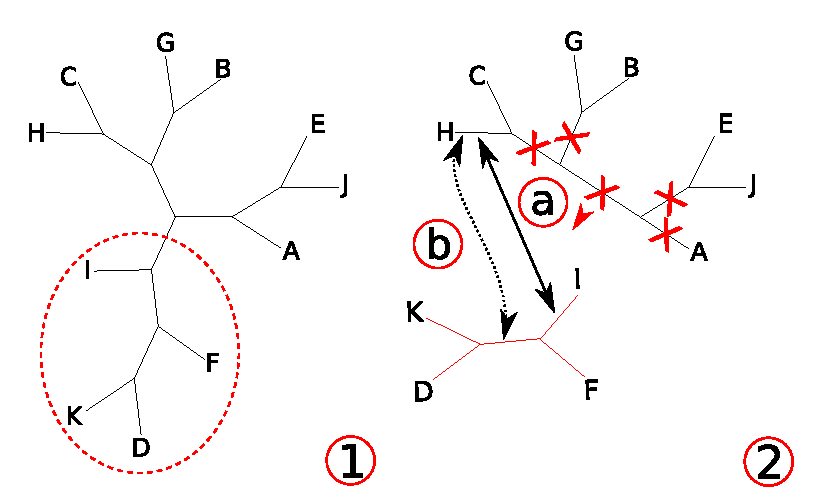
\includegraphics[width=0.9\textwidth]{Figure/TBR_modif.pdf}
\caption{Generalised TBR. \textbf{1}: the trees are split at a random edge and both subtrees are unrooted; \textbf{2a}: the red tree is then rooted on the edge closest to the bisection edge and reconnected to an edge on the black tree (i.e. a SPR move); \textbf{2b}: the red tree is rooted on any of its edges and reconnected to an edge on the black tree (i.e. a TBR move). Note that in both cases, the red tree can not be reconnected on the edge of origin (indicated by the red arrow) nor on any of the adjacent edges (marked with a red cross) to avoid any redundant tree rearrangements.}
\label{Figure_TBR_modif}
\end{figure}

We believe that such consideration of the SPR algorithm as a constrained TBR highly facilitates both algorithm's implementation.
In fact, in this case only one algorithm needs to be implemented with one mandatory restricting rules (no reconnection on the bisection edge and it's neighbours) and an optional restriction that can be activate or not to create either TBR or SPR (respectively rerooting on any edge or only on the bisection one).
This approach is not different than the classic SPR and TBR algorithms described in the literature \citep{allen2001subtree,felsenstein2004inferring} but proposes an easier implementation.

One of the major concern in phylogenetic inference, during the tree search phase is to evenly (or at worst, randomly) sample the tree space but without spending to much time sampling all possible topologies.
This allows to identify the different topology islands where the tree search must be focused in order to find the optimal topology.
One solution to achieve this it to shift between tree rearrangement algorithms during the tree search: first, using an algorithm allowing bold tree rearrangements to explore the overall tree space and then a more conservative one to do a ``fine grain'' search in local optima \citep{lakner2008efficiency}.
This joint SPR-TBR implementation could easily allow such tree rearrangement shifts by switching between the different restriction rules without implementing different algorithms.
For example, one could first allow the algorithm to reroot the bissected tree randomly on each of it's edges, creating bolder rearrangements (i.e. exploring the overall tree space) and the constrict the algorithm to only reroot the tree on the edge closest to the bisection edge, creating ``finer grain'' search (i.e. exploring only the SPR island).


\section{Acknowledgments}
European Research Council under the European Union’s Seventh Framework Programme (FP/2007–2013)/ERC Grant Agreement number 311092.


\bibliographystyle{sysbio}
\bibliography{References}

\end{document}

